\documentclass[pdftex,12pt,letter]{article}
\usepackage{fancyhdr}
\usepackage{enumerate}
\usepackage{tabularx}
\usepackage{graphicx}
\usepackage{array}
\usepackage{hyperref}
\usepackage[justification=justified,singlelinecheck=false]{caption}
\usepackage{placeins}
\usepackage{rotating}
\makeatletter
  \renewcommand\@seccntformat[1]{\csname the#1\endcsname.\quad}
\makeatother

\newcolumntype {Y}{ >{\raggedright \arraybackslash }X}
\newcommand{\HRule}{\rule{\linewidth}{0.5mm}}
\captionsetup{labelformat=empty}

\begin{document}

\begin{titlepage}
\begin{flushright}
\HRule \\[0.4cm]
{ \bfseries
{\huge CWRUtility Bug Reports\\[1cm]}
{\Large for\\[1cm]}
{\huge CWRUtility\large\\[4cm]}
{\large Prepared by\\Jason Kuster\\[1cm]
Version 1.0\\[1cm]
KOALAA Development\\[1cm]
December 7, 2012}}
\end{flushright}
\end{titlepage}
\begin{table}[!t]
\caption*{\bfseries Revision History}
\begin{tabularx}{\textwidth }[t]{|l|Y|Y|l|}
\hline
\bfseries Name & \bfseries Date & \bfseries Reasons for Change & \bfseries Version \\ \hline
Kuster & 12/6/2012 & Initial Draft & 1.0\\
\hline
\end{tabularx}
\end{table}
\FloatBarrier
\newpage
\clearpage
\section{Introduction}
For unit tests, we used the built-in Windows Phone unit test framework which takes user-defined tests and incorporates them into a phone application. That application than can be run to execute all of the tests. As shown below, the results of the tests will be displayed on the phone, including informative error message in the case of test failure.
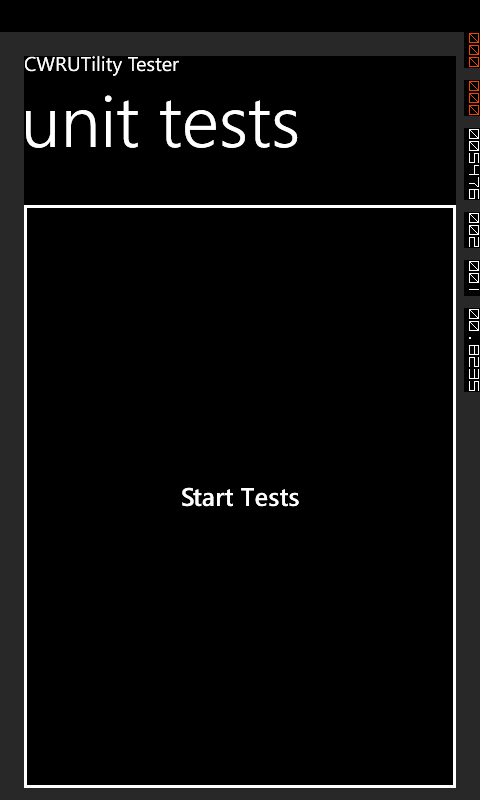
\includegraphics[width=4in]{ss1.png}
\FloatBarrier
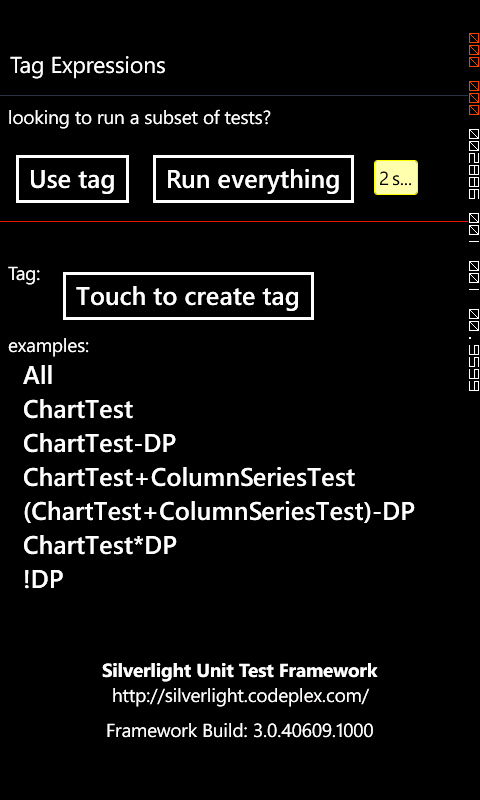
\includegraphics[width=4in]{ss2.png}
\FloatBarrier
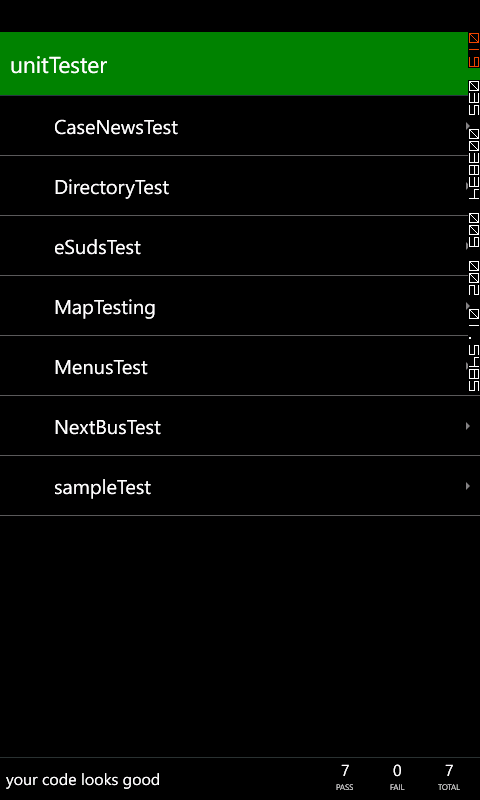
\includegraphics[width=4in]{ss3.png}
\FloatBarrier
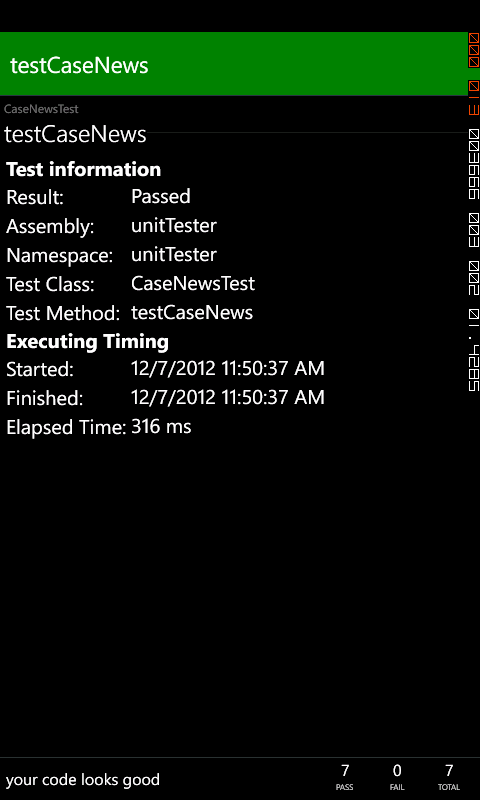
\includegraphics[width=4in]{ss4.png}
\FloatBarrier
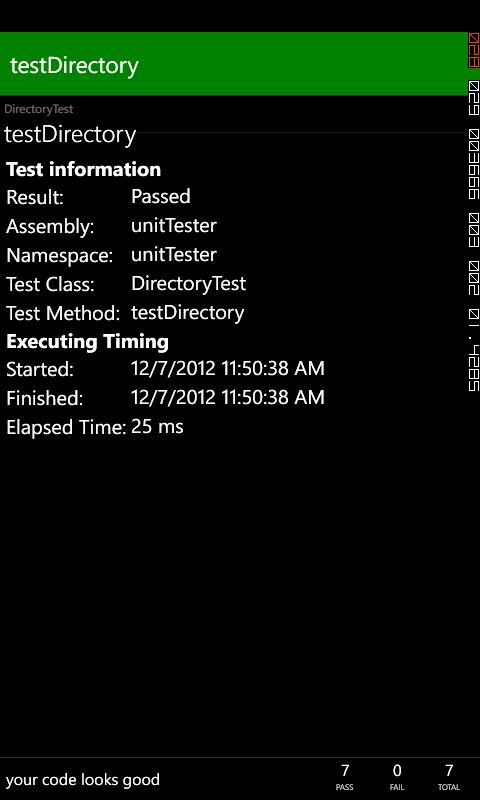
\includegraphics[width=4in]{ss5.png}
\FloatBarrier
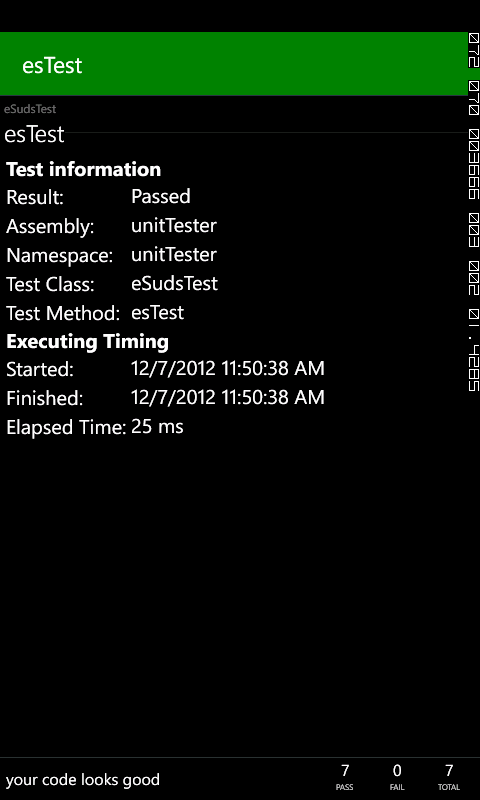
\includegraphics[width=4in]{ss6.png}
\FloatBarrier
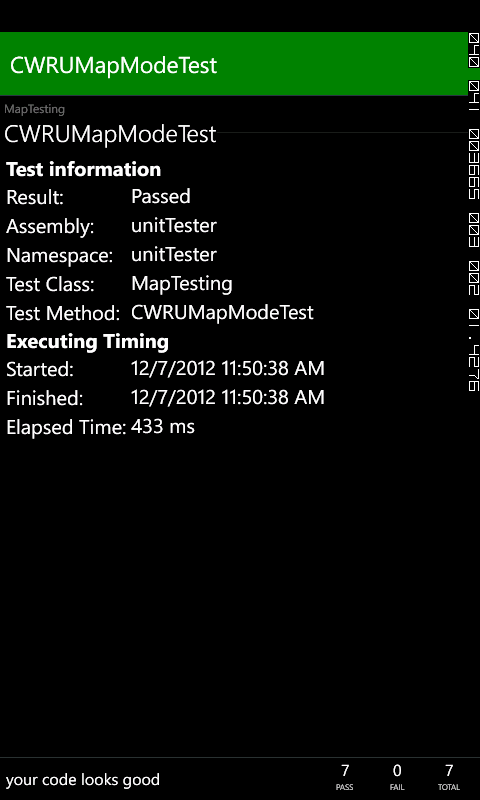
\includegraphics[width=4in]{ss7.png}
\FloatBarrier
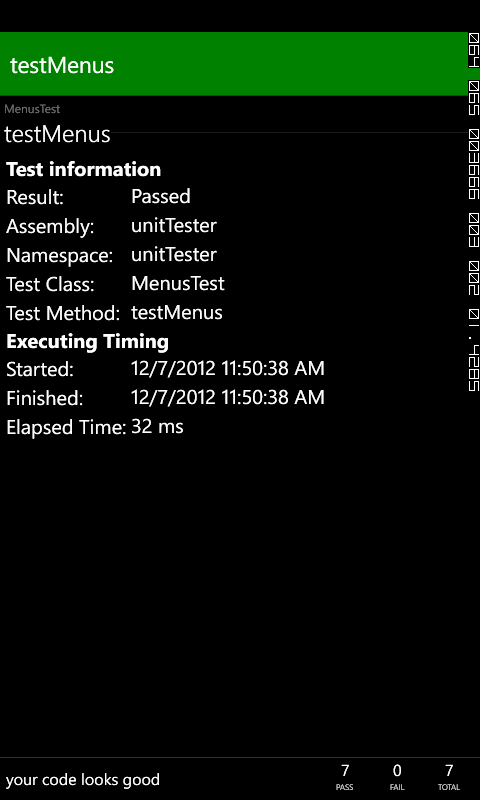
\includegraphics[width=4in]{ss8.png}
\FloatBarrier
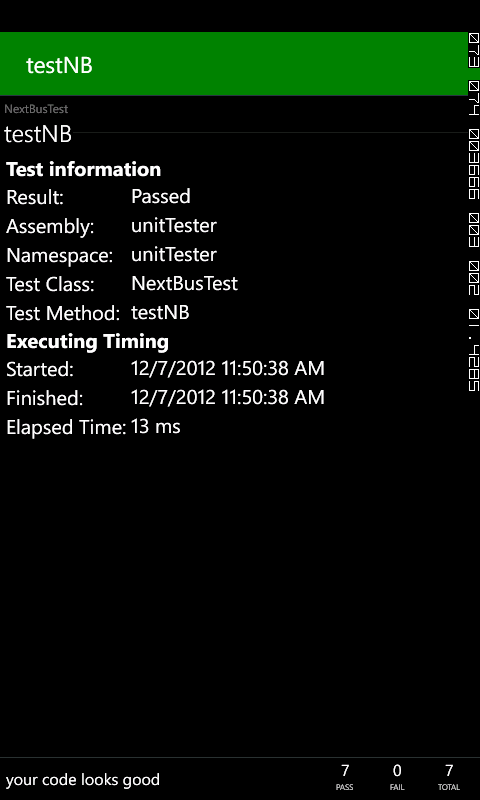
\includegraphics[width=4in]{ss9.png}
\FloatBarrier

\end{document}